%! Author = Sujal Singh
%! Date = 3/25/26

% Preamble
\documentclass[11pt]{beamer}

\title{Case Study on Online Shopping System}
\author[Vatsal, Pranav, Sujal, Parikshit]
{\(|\) Vatsal Kumar \(|\) Pranav Bisht \(|\) Sujal Singh \(|\) Parikshit Pandey \(|\)}
\date[0\{21,27,41,59\}19051723]{\textbf{Enrollment Numbers:\\}\texttt{0\{21,27,41,59\}19051723}}


% Packages
\usepackage{amsmath}
\usepackage{xcolor}
\usepackage{tikz}
\usepackage{tabularray}
\usepackage{pgfgantt}

\usetikzlibrary{shapes,arrows,arrows.meta,positioning}

\usetheme{Madrid}
\setbeamertemplate{navigation symbols}{}
\setbeamertemplate{frametitle continuation}[from second][]

% Document
\begin{document}
    \begin{frame}{Case Study on Online Shopping System}
        \begin{center}
            %! suppress = FileNotFound
            
\includegraphics[width=80pt]{logo}
        \end{center}
        \maketitle
    \end{frame}

    \begin{frame}[allowframebreaks]{Introduction}
        \begin{columns}
            \begin{column}{0.65\textwidth}
                An online shopping system enables users to purchase products over the internet without visiting physical
                stores. It integrates components like product catalogs, payment systems, and order processing to deliver
                a seamless shopping experience.

                \begin{itemize}
                    \item Allows users to browse, search, and purchase products online
                    \item Provides features like shopping cart, order tracking, and payments
                    \item Supports multiple users simultaneously
                    \item Reduces operational cost compared to traditional retail
                \end{itemize}
            \end{column}
            \begin{column}{0.35\textwidth}
                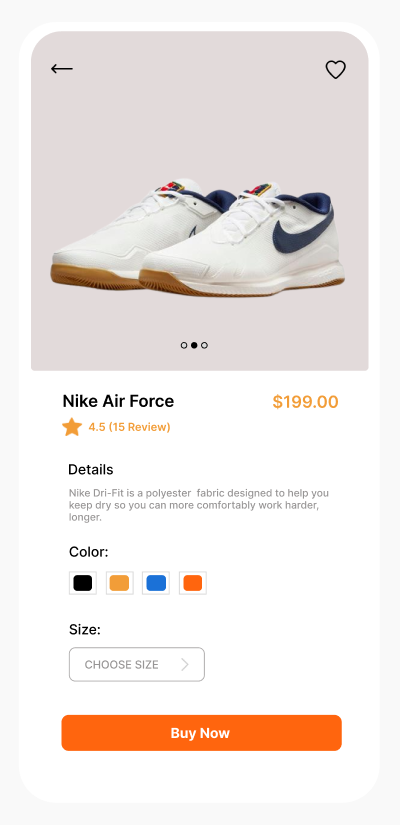
\includegraphics[width=\textwidth]{ui}
            \end{column}
        \end{columns}


        \framebreak

        \vspace{-10pt}
        \textbf{Project as a System:}\\[10pt]

        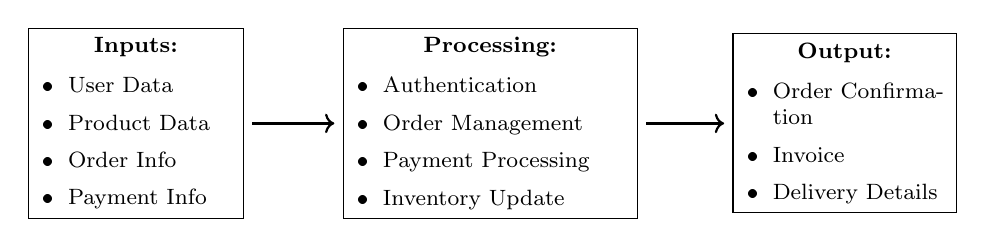
\begin{tikzpicture}
            [node distance = 4.5cm, font=\footnotesize, execute at begin node={\setlength{\leftmargini}{1.3em}}]
            \node[draw, rectangle, text width=2.5cm, align=center] (input) {
                \textbf{Inputs:}\\
                \begin{itemize}
                    \item User Data
                    \item Product Data
                    \item Order Info
                    \item Payment Info
                \end{itemize}
            };
            \node[draw, rectangle, text width=3.5cm, align=center, right of=input] (process) {
                \textbf{Processing:}\\
                \begin{itemize}
                    \item Authentication
                    \item Order Management
                    \item Payment Processing
                    \item Inventory Update
                \end{itemize}
            };
            \node[draw, rectangle, text width=2.6cm, align=center, right of=process] (output) {
                \textbf{Output:}\\
                \begin{itemize}
                    \item Order Confirmation
                    \item Invoice
                    \item Delivery Details
                \end{itemize}
            };

            \draw[->, thick, shorten >=3pt, shorten <= 3pt] (input) -- (process);
            \draw[->, thick, shorten >=3pt, shorten <= 3pt] (process) -- (output);
        \end{tikzpicture}

        \framebreak

        \textbf{Scope:}\\
        \begin{itemize}
            \item Online product browsing and search
            \item Order placement and tracking
            \item Payment processing integration
            \item Basic admin and inventory management
        \end{itemize}

        \\~\\

        \textbf{Objective:}\\
        \begin{itemize}
            \item Provide fast and reliable service
            \item Ensure secure transactions
            \item Support multiple concurrent users
            \item Minimize system response time
        \end{itemize}

    \end{frame}

    \begin{frame}{Process Model}
        \textbf{Waterfall Phases (with timeline):}\\
        \begin{center}
            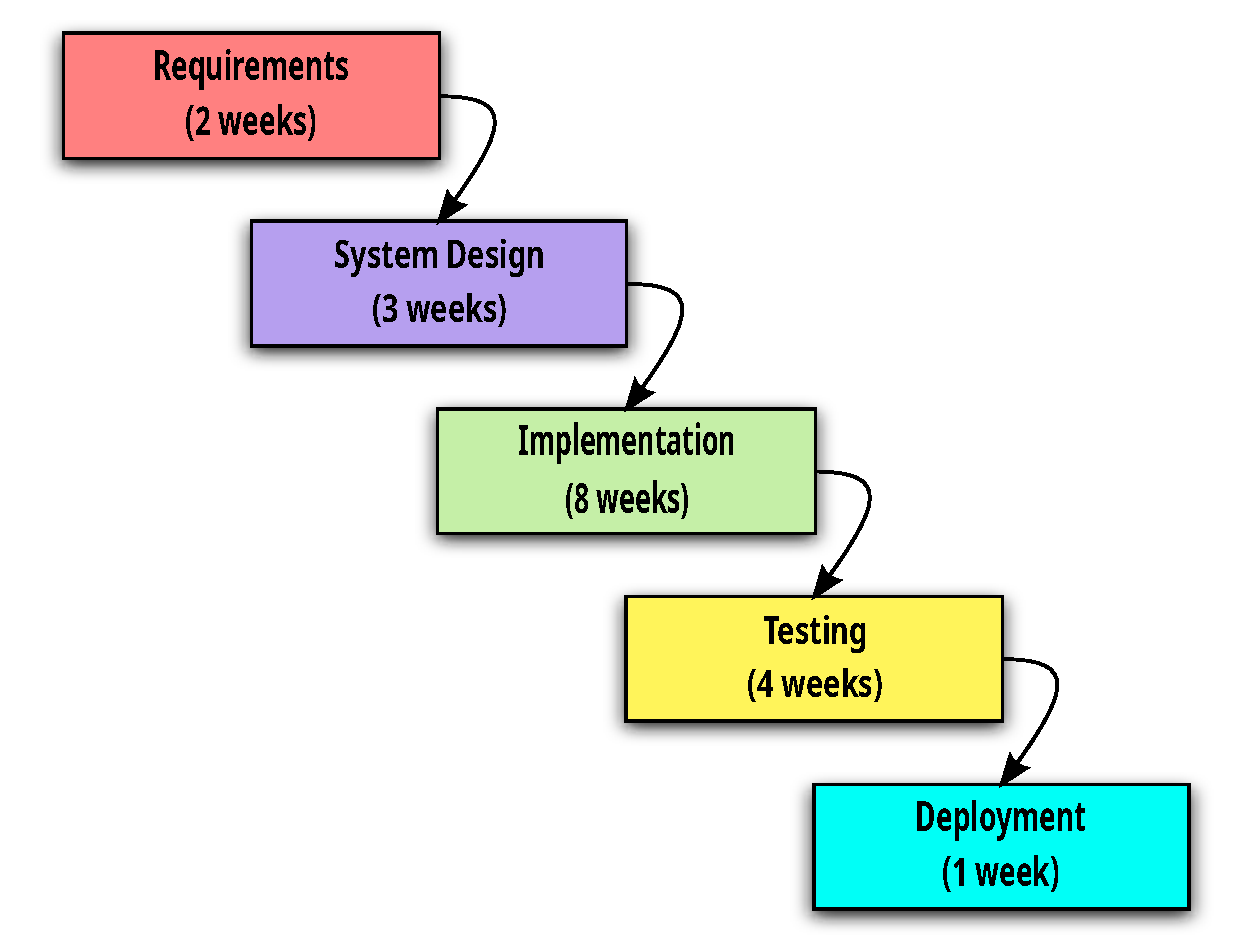
\includegraphics[width=0.7\textwidth]{timeline}
        \end{center}
    \end{frame}

    \begin{frame}[t, allowframebreaks]{Project Planning}
        \textbf{Work Breakdown Structure:}\\[10pt]

        \vfill
        \small
        \begin{tabular}{|c|c|c|}
            \hline
            \textbf{Level 1}     & \textbf{Level 2}      & \textbf{Level 3}         \\
            \hline

            Requirement Analysis & Requirement Gathering & User needs, Market study \\
            & Specification         & SRS documentation        \\
            \hline

            System Design        & Data Design           & Product DB, User DB      \\
            & Interface Design      & UI/UX layout             \\
            \hline

            Development          & Frontend              & UI pages, Cart system    \\
            & Backend               & Business logic, APIs     \\
            \hline

            Testing              & Unit Testing          & Module testing           \\
            & Integration Testing   & System testing           \\
            \hline

            Deployment           & Deployment Setup      & Server configuration     \\
            & Maintenance           & Updates, Bug fixes       \\
            \hline

        \end{tabular}
        \vfill

        \framebreak

        \textbf{CPM:}\\[10pt]


        \begin{tabular}{|c|c|}
            \hline
            \textbf{Activity} & \textbf{Duration (weeks)} \\
            \hline
            Requirement       & 2                         \\
            \hline
            Design            & 3                         \\
            \hline
            Development       & 8                         \\
            \hline
            Testing           & 4                         \\
            \hline
            Deployment        & 1                         \\
            \hline
        \end{tabular}

        \\[20pt]

        \begin{tikzpicture}[font=\footnotesize,scale=0.85, transform shape]
            \node[text width=65pt, align=center] (requirement) {
                \begin{tblr}{width=\textwidth,colspec={|X[1,c]|X[1,c]|X[1,c]|}}
                    \hline
                    0 & 2 & 2\\
                    \hline
                    \SetCell[c=3]{c} Requirements \\
                    \hline
                    0 & 0 & 2 \\
                    \hline
                \end{tblr}
            }

            \node[text width=50pt, align=center, right=15pt of requirement] (design) {
                \begin{tblr}{width=\textwidth,colspec={|X[1,c]|X[1,c]|X[1,c]|}}
                    \hline
                    2 & 3 & 5\\
                    \hline
                    \SetCell[c=3]{c} Design \\
                    \hline
                    2 & 0 & 5 \\
                    \hline
                \end{tblr}
            }

            \node[text width=60pt, align=center, right=15pt of design] (development) {
                \begin{tblr}{width=\textwidth,colspec={|X[1,c]|X[1,c]|X[1,c]|}}
                    \hline
                    5 & 8 & 13 \\
                    \hline
                    \SetCell[c=3]{c} Development \\
                    \hline
                    5 & 0 & 13\\
                    \hline
                \end{tblr}
            }

            \node[text width=60pt, align=center, right=20pt of development] (testing) {
                \begin{tblr}{width=\textwidth,colspec={|X[1,c]|X[1,c]|X[1,c]|}}
                    \hline
                    13 & 4 & 17 \\
                    \hline
                    \SetCell[c=3]{c} Testing \\
                    \hline
                    13 & 0 & 17 \\
                    \hline
                \end{tblr}
            }

            \node[text width=60pt, align=center, right=20pt of testing] (deployment) {
                \begin{tblr}{width=\textwidth,colspec={|X[1,c]|X[1,c]|X[1,c]|}}
                    \hline
                    17 & 1 & 18 \\
                    \hline
                    \SetCell[c=3]{c} Deployment \\
                    \hline
                    17 & 0 & 18 \\
                    \hline
                \end{tblr}
            }

            \draw[-{Triangle}, thick] (requirement) -- (design);
            \draw[-{Triangle}, thick] (design) -- (development);
            \draw[-{Triangle}, thick, shorten <=3pt] (development) -- (testing);
            \draw[-{Triangle}, thick] (testing) -- (deployment);
        \end{tikzpicture}

        \vfill

        \textbf{Total Time = 18 weeks. \\ No slack, delay in any task delays the whole project.}

        \framebreak

        \textbf{PERT Analysis:}

        \\[20pt]

        \scriptsize
        \setlength{\tabcolsep}{1.25em} % for the horizontal padding
        {\renewcommand{\arraystretch}{1.8}% for the vertical padding
            \begin{tabular}{|c|c|c|c|c|c|}
                \hline
                \textbf{Activity} & \textbf{O} & \textbf{M} & \textbf{P} & \textbf{Calculation} & \textbf{TE} \\
                \hline
                Requirement       & 1          & 2          & 3          & (1 + 8 + 3)/6        & 2.00        \\
                \hline
                Design            & 2          & 3          & 4          & (2 + 12 + 4)/6       & 3.00        \\
                \hline
                Development       & 6          & 8          & 10         & (6 + 32 + 10)/6      & 8.00        \\
                \hline
                Testing           & 3          & 4          & 5          & (3 + 16 + 5)/6       & 4.00        \\
                \hline
                Deployment        & 1          & 1          & 2          & (1 + 4 + 2)/6        & 1.17        \\
                \hline
                \multicolumn{5}{|c|}{\textbf{Total Time = $\sum TE =$}} & \textbf{18.17} \\
                \hline
            \end{tabular}
        }

        \framebreak

        \textbf{\large Gantt Chart:}

        \\[20pt]
        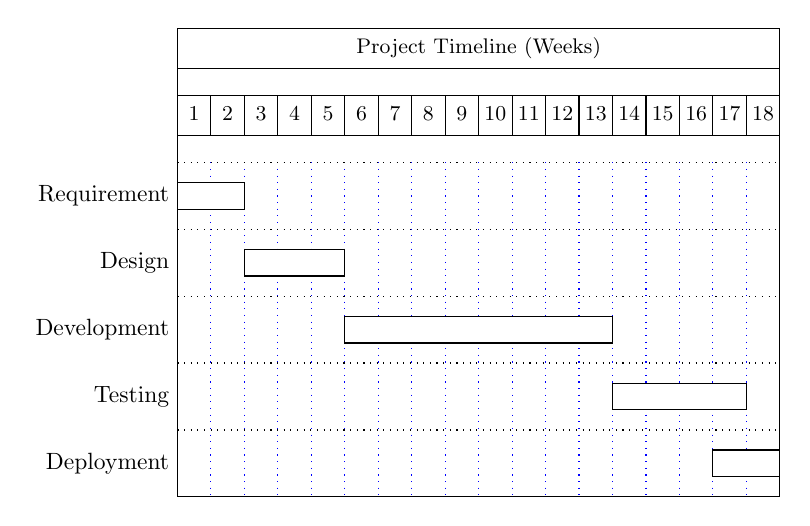
\begin{tikzpicture}[scale=0.85, transform shape]
        \begin{ganttchart}[
            hgrid=true,
            vgrid={*1{blue, dotted}},
            expand chart=\textwidth
        ]{1}{18}
            \gantttitle{Project Timeline (Weeks)}{18}\\
            \gantttitlelist{1,...,18}{1}\\
            \ganttbar{Requirement}{1}{2} \\
            \ganttbar{Design}{3}{5}\\
            \ganttbar{Development}{6}{13}\\
            \ganttbar{Testing}{14}{17}\\
            \ganttbar{Deployment}{17}{18}
        \end{ganttchart}
        \end{tikzpicture}

        \framebreak

        \textbf{\large Cost-Benefit Analysis:}

        \\[10pt]

        \textbf{Cost Components:}
        \begin{itemize}
            \item Development Cost: ₹6,00,000
            \item Infrastructure Cost: ₹3,00,000
            \item Operational Cost: ₹2,00,000
        \end{itemize}

        \vspace{0.3cm}

        \textbf{Total Cost:} ₹11,00,000

        \vspace{0.5cm}

        \textbf{Annual Revenue:} ₹8,00,000 \\
        \textbf{Operational Cost (Yearly):} ₹2,00,000 \\

        \vspace{0.3cm}

        \textbf{Net Annual Benefit:} ₹6,00,000

        \vspace{0.5cm}

        \textbf{Payback Period:}
        \[
            \frac{11,00,000}{6,00,000} \approx 1.83 \text{ years}
        \]


        \framebreak

        \textbf{Net Present Value (NPV):}

        \[
            NPV = \sum \frac{B_t}{(1 + r)^t} - C
        \]

        \textbf{Assumptions:}
        \begin{itemize}
            \item Annual Benefit = ₹6,00,000
            \item Discount Rate (r) = 10\%
            \item Duration = 3 years
        \end{itemize}

        \vspace{0.3cm}

        \textbf{Present Value of Benefits:}
        \begin{itemize}
            \item Year 1: ₹5,45,455
            \item Year 2: ₹4,95,868
            \item Year 3: ₹4,50,789
        \end{itemize}

        \textbf{Total PV = ₹14,92,112}

        \vspace{0.3cm}

        \textbf{NPV = 14,92,112 − 11,00,000 = ₹3,92,112 (Positive)}

        \vspace{0.5cm}

        \textbf{Return on Investment (ROI):}
        \[
            ROI = \frac{\text{Net Profit}}{\text{Total Cost}} \times 100 \approx 54\%
        \]

        \framebreak

        \textbf{\large Risk Analysis:}

        \\[20pt]

        \centering
        \small
        \begin{tblr}{width=\textwidth,colspec={|c|c|c|p{4cm}|}}
            \hline
            \textbf{Risk}      & \textbf{Probability} & \textbf{Impact} & \textbf{Mitigation}                   \\
            \hline
            Server Downtime    & Medium               & High            & Use backup servers and monitoring     \\
            \hline
            Payment Failure    & High                 & Medium          & Retry mechanism and multiple gateways \\
            \hline
            Data Breach        & Low                  & Very High       & Encryption and secure authentication  \\
            \hline
            Inventory Mismatch & Medium               & Medium          & Real-time inventory updates           \\
            \hline
            Delivery Delays    & High                 & Medium          & Optimize logistics and tracking       \\
            \hline
        \end{tblr}
    \end{frame}

    \begin{frame}{The End.}
        \vfill
        \begin{center}
            \textbf{\Huge Thank you.}
        \end{center}
        \vfill
    \end{frame}
\end{document}
